%%%%% Set up %%%%%

% Set document style and font size
\documentclass[12pt]{article}\usepackage[]{graphicx}\usepackage[]{color}
%% maxwidth is the original width if it is less than linewidth
%% otherwise use linewidth (to make sure the graphics do not exceed the margin)
\makeatletter
\def\maxwidth{ %
  \ifdim\Gin@nat@width>\linewidth
    \linewidth
  \else
    \Gin@nat@width
  \fi
}
\makeatother

\definecolor{fgcolor}{rgb}{0.345, 0.345, 0.345}
\newcommand{\hlnum}[1]{\textcolor[rgb]{0.686,0.059,0.569}{#1}}%
\newcommand{\hlstr}[1]{\textcolor[rgb]{0.192,0.494,0.8}{#1}}%
\newcommand{\hlcom}[1]{\textcolor[rgb]{0.678,0.584,0.686}{\textit{#1}}}%
\newcommand{\hlopt}[1]{\textcolor[rgb]{0,0,0}{#1}}%
\newcommand{\hlstd}[1]{\textcolor[rgb]{0.345,0.345,0.345}{#1}}%
\newcommand{\hlkwa}[1]{\textcolor[rgb]{0.161,0.373,0.58}{\textbf{#1}}}%
\newcommand{\hlkwb}[1]{\textcolor[rgb]{0.69,0.353,0.396}{#1}}%
\newcommand{\hlkwc}[1]{\textcolor[rgb]{0.333,0.667,0.333}{#1}}%
\newcommand{\hlkwd}[1]{\textcolor[rgb]{0.737,0.353,0.396}{\textbf{#1}}}%
\let\hlipl\hlkwb

\usepackage{framed}
\makeatletter
\newenvironment{kframe}{%
 \def\at@end@of@kframe{}%
 \ifinner\ifhmode%
  \def\at@end@of@kframe{\end{minipage}}%
  \begin{minipage}{\columnwidth}%
 \fi\fi%
 \def\FrameCommand##1{\hskip\@totalleftmargin \hskip-\fboxsep
 \colorbox{shadecolor}{##1}\hskip-\fboxsep
     % There is no \\@totalrightmargin, so:
     \hskip-\linewidth \hskip-\@totalleftmargin \hskip\columnwidth}%
 \MakeFramed {\advance\hsize-\width
   \@totalleftmargin\z@ \linewidth\hsize
   \@setminipage}}%
 {\par\unskip\endMakeFramed%
 \at@end@of@kframe}
\makeatother

\definecolor{shadecolor}{rgb}{.97, .97, .97}
\definecolor{messagecolor}{rgb}{0, 0, 0}
\definecolor{warningcolor}{rgb}{1, 0, 1}
\definecolor{errorcolor}{rgb}{1, 0, 0}
\newenvironment{knitrout}{}{} % an empty environment to be redefined in TeX

\usepackage{alltt}

% File path to resources (style file etc)
\newcommand{\locRepo}{csas-style}

% Style file for DFO Technical Reports
\usepackage{\locRepo/tech-report}

% header-includes from R markdown entry
\usepackage{pdflscape}

%%%%% Variables %%%%%

% New definitions: Title, year, report number, authors
% Protect lower case words (i.e., species names) in \Addlcwords{}, in "TechReport.sty"
\newcommand{\trTitle}{Results of sablefish (\emph{Anoplopoma fimbria}) head measurement study, putting our noggins together.}
\newcommand{\trYear}{2020}
\newcommand{\trReportNum}{nnn}
% Optional
\newcommand{\trAuthFootA}{Email: \href{mailto:Kathryn.Temple@dfo-mpo.gc.ca}{\nolinkurl{Kathryn.Temple@dfo-mpo.gc.ca}} \textbar{} telephone: (250) 756-xxxx}
\newcommand{\trAuthsLong}{Kathryn x. Temple, Lisa C. Lacko and B C}
\newcommand{\trAuthsBack}{Kathryn x. Temple and Lacko, L.C. and B.C.}

% New definition: Address
\newcommand{\trAddy}{Pacific Biological Station\\
Fisheries and Oceans Canada, 3190 Hammond Bay Road\\
Nanaimo, British Columbia, V9T 6N7, Canada\\}

% Abstract
\newcommand{\trAbstract}{This document describes sampling activities and summarizes results}

% Resume (i.e., French abstract)
\newcommand{\trResume}{}

\newcommand{\trISBN}{}

%%%%% Start %%%%%

% Start the document
\IfFileExists{upquote.sty}{\usepackage{upquote}}{}
\begin{document}

%%%% Front matter %%%%%

% Add the first few pages
\frontmatter

%%%%% Drafts %%%%%

%\linenumbers  % Line numbers
%\onehalfspacing  % Extra space between lines
\renewcommand{\headrulewidth}{0.5pt}  % Header line
\renewcommand{\footrulewidth}{0.5pt}  % footer line
%\pagestyle{fancy}\fancyhead[c]{Draft: Do not cite or circulate}  % Header text

%%%%% Main document %%%%%
\hypertarget{introduction}{%
\section{Introduction}\label{introduction}}

The tag and release study has been conducted annually since 1991. Whole tagged fish are recovered mainly in the commercial fishery (trap, trawl, hook and line) and processed at the point of landing through the Dockside Monitoring Program (DMP) currently operated by Archipelago Marine Research (AMR). In order to eliminate whole fish samples, we assessed whether sablefish fork length and weight could be predicted from 6 different head dimension measurements. Simple linear regression models were calculated from 431 specimens collected on the 2016 WCVI and WCHG surveys using a length stratified sampling protocol.

\hypertarget{methods}{%
\section{Methods}\label{methods}}

Sablefish head morphometric project: Summary Mar 15, 2017.
\begin{enumerate}
\def\labelenumi{\arabic{enumi}.}
\item
  431 Sablefish heads were collected on the 2016 WCVI and WCHG surveys using a trip-wide length stratified sampling protocol.
\item
  The 438 heads measured were from fish that ranged from 240-1080 mm fork length. 212 were collected on trip 79190 (WCVI), and 219 were from trip 80378 (WCHG). In addition to measuring the head dimensions as described below, we collected tissue for DNA analysis (small fin clips collected in to 95\% Ethanol) from the first 138 fish measured, and otoliths from every specimen (excluding the 7 small sablefish collected on the salmon survey).
\item
  Definition of 6 head dimensions measured and instructions for positioning the calipers (Table~\ref{tab:table1}).
\item
  Each measurement was ranked in terms of `Ease of Use' and `Repeatability'
\end{enumerate}
\clearpage

\hypertarget{results}{%
\section{Results}\label{results}}

The mean values of the predictor variables were \ldots\ldots\ldots.. (Table~\ref{tab:table2}).\\
The top ranked measurement in terms of `Ease of Use' and `Repeatability' was Interorbital distance (Table~\ref{tab:table3}).

We found evidence of relationships between upper jaw length and fork length (p = \ensuremath{9.358\times 10^{-278}}) ; eye diameter and fork length (p = \ensuremath{5.34\times 10^{-203}}); interorbital distance and fork length (p = \ensuremath{5.539\times 10^{-272}} ); upper snout length and fork length (p = \ensuremath{4.593\times 10^{-292}}); postorbital to preoperculum length and fork length (p = \ensuremath{2.024\times 10^{-247}}); and postorbital head length and fork length (p = 0).

The estimated slope is 7.695 (SE 0.088) units of fork length per unit of upper jaw length; the estimated slope is 21.994 (SE 0.389) units of fork length per unit of eye diameter; the estimated slope is 11.622 (SE 0.138) units of fork length per unit of interorbital distance; the estimated slope is 11.182 (SE 0.118 units of fork length per unit of snout length; the estimated slope is 14.373 (SE 0.191) units of fork length per unit of postorbital to preoperculum length; and the estimated slope is 6.83 (SE 0.185) units of fork length per unit of postorbital head length.

\hypertarget{tables}{%
\section{Tables}\label{tables}}



\begin{table}

\caption{\label{tab:table1}Definition of head dimensions measured and instructions for positioning the calipers. ~\\
\hspace*{0.333em}\\}
\centering
\fontsize{8}{10}\selectfont
\begin{tabular}[t]{>{\raggedright\arraybackslash}p{2.2cm}>{\raggedright\arraybackslash}p{2.7cm}>{\raggedright\arraybackslash}p{4.7cm}}
\toprule
Measurement.type & Head.dimensions & Instructions.for.positioning.calipers\\
\midrule
Upper jaw length & tip of snout to the posterior edge of the maxilla & Measure from the most forward point/centre of the snout to the back of the maxilla.\\
\hline
Eye diameter & anterior-posterior diameter of eye socket & Use the outward-facing points of the calipers. Stretch them firmly against the eye socket at the vertical midpoint of the eye\\
\hline
InterOrbital distance & narrowest distance between eye sockets, measured on dorsal surface & Measure at the horizontal midpoint of the eyes on the dorsal surface.\\
\hline
Snout length & tip of snout to anterior inner edge of eye socket & Measure from the most forward point/centre of the snout, to the horizontal midpoint of the anterior edge of the eye socket\\
\hline
Post orbital to preoperculum distance & posterior inner edge of orbit to visual insertion point of preopercle & Measure from the back of the eye socket (caliper vertically centred), to the preopercle.  Lift the preopercle away from the fish slightly so that you can see the preopercle bone underneath the skin. Measure to the point at which you can see the preopercle bone insertion point (this will be underneath the skin and won’t necessarily be where the gill slit ends.\\
\hline
Post orbital head length & posterior inner edge of orbit to dorsal insertion of opercle & Measure from the back of the eye socket (caliper vertically centred), to the ‘gill cover notch’ at the dorsal insertion of the opercle.  Hold the operculum taut and measure to the bone underneath the gill cover notch rather than to the flap of skin that forms the notch itself.\\
\bottomrule
\end{tabular}
\end{table}

\begin{table}

\caption{\label{tab:table2}Table of sample size, mean and standard deviation for predictor and response variables.}
\centering
\fontsize{8}{10}\selectfont
\begin{tabular}[t]{>{\raggedright\arraybackslash}p{3.7cm}>{\raggedright\arraybackslash}p{0.6cm}>{\raggedright\arraybackslash}p{0.6cm}>{\raggedright\arraybackslash}p{0.6cm}>{\raggedright\arraybackslash}p{2.1cm}>{\raggedright\arraybackslash}p{0.8cm}>{\raggedright\arraybackslash}p{0.6cm}}
\toprule
Predictor variable & n & mean & sd & Response variable & mean & sd\\
\midrule
Upper jaw length & 437 & 57.953 & 15.223 & Fork length & 573.272 & 120.435\\
Eye diameter & 438 & 25.902 & 5.132 & Fork length & 573.299 & 120.299\\
InterOrbital distance & 437 & 40.373 & 10.06 & Fork length & 573.364 & 120.429\\
Snout length & 437 & 44.814 & 10.517 & Fork length & 573.272 & 120.435\\
Post orbital to preoperculum length & 426 & 31.495 & 8.022 & Fork length & 571.338 & 119.54\\
Post orbital head length & 130 & 60.852 & 18.868 & Fork length & 566.462 & 134.805\\
\bottomrule
\end{tabular}
\end{table}

\begin{table}

\caption{\label{tab:table3}Ease of use and repeatability considerations for each measurement.}
\centering
\fontsize{8}{10}\selectfont
\begin{tabular}[t]{>{\raggedright\arraybackslash}p{1.6cm}>{\raggedleft\arraybackslash}p{0.6cm}>{\raggedright\arraybackslash}p{0.6cm}>{\raggedleft\arraybackslash}p{1.7cm}>{\raggedleft\arraybackslash}p{1.2cm}>{\raggedright\arraybackslash}p{3.7cm}}
\toprule
Measurement & N & R & Ease.of.use & Repeatability & Considerations\\
\midrule
Upper jaw length & 437 & 0.946 & 3 & 4 & Bony part; can measure on right or left side.  Electronic Calipers tended to malfunction when longer measurements attempted; had to use manual calipers for >15cm distances; somewhat awkward to measure. The end of the maxilla can be hard to define. Must ensure caliper is in center of snout\\
\hline
Eye diameter & 438 & 0.88 & 3 & 2 & Easy to define where to hold the calipers in the eye socket, but the tissue is soft/stretchy so its difficult to know how hard to press against the flesh; can measure on right or left side. Uses the outside rather than the inside of the calipers (? slower); Soft tissue so repeatability is questionable; somewhat awkward to measure\\
\hline
Interorbital distance & 437 & 0.943 & 5 & 5 & Bony part;  Easy to define where to hold calipers; so far there has been no reason (eg damage) to not include this measurement\\
\hline
Snout length & 437 & 0.954 & 4 & 5 & Bony part; can measure on right or left side; must ensure caliper is in centre of snout\\
\hline
Post orbital to pre-operculum & 426 & 0.93 & 4 & 5 & Bony part; can measure on right or left side.  Maybe need to improve definition of instruction of where to hold caliper on pre-operculum\\
\hline
Post orbital head length & 130 & 0.914 & 3 & 2 & Can measure on right or left side. Operculum was cut off on some fish, likely to be cut off on commercially caught fish. Electronic Calipers tended to malfunction when longer measurements attempted; had to use manual calipers for >15 cm distances\\
\bottomrule
\end{tabular}
\end{table}
\clearpage

\hypertarget{figures}{%
\section{Figures}\label{figures}}


\begin{figure}[htb]

{\centering \pdftooltip{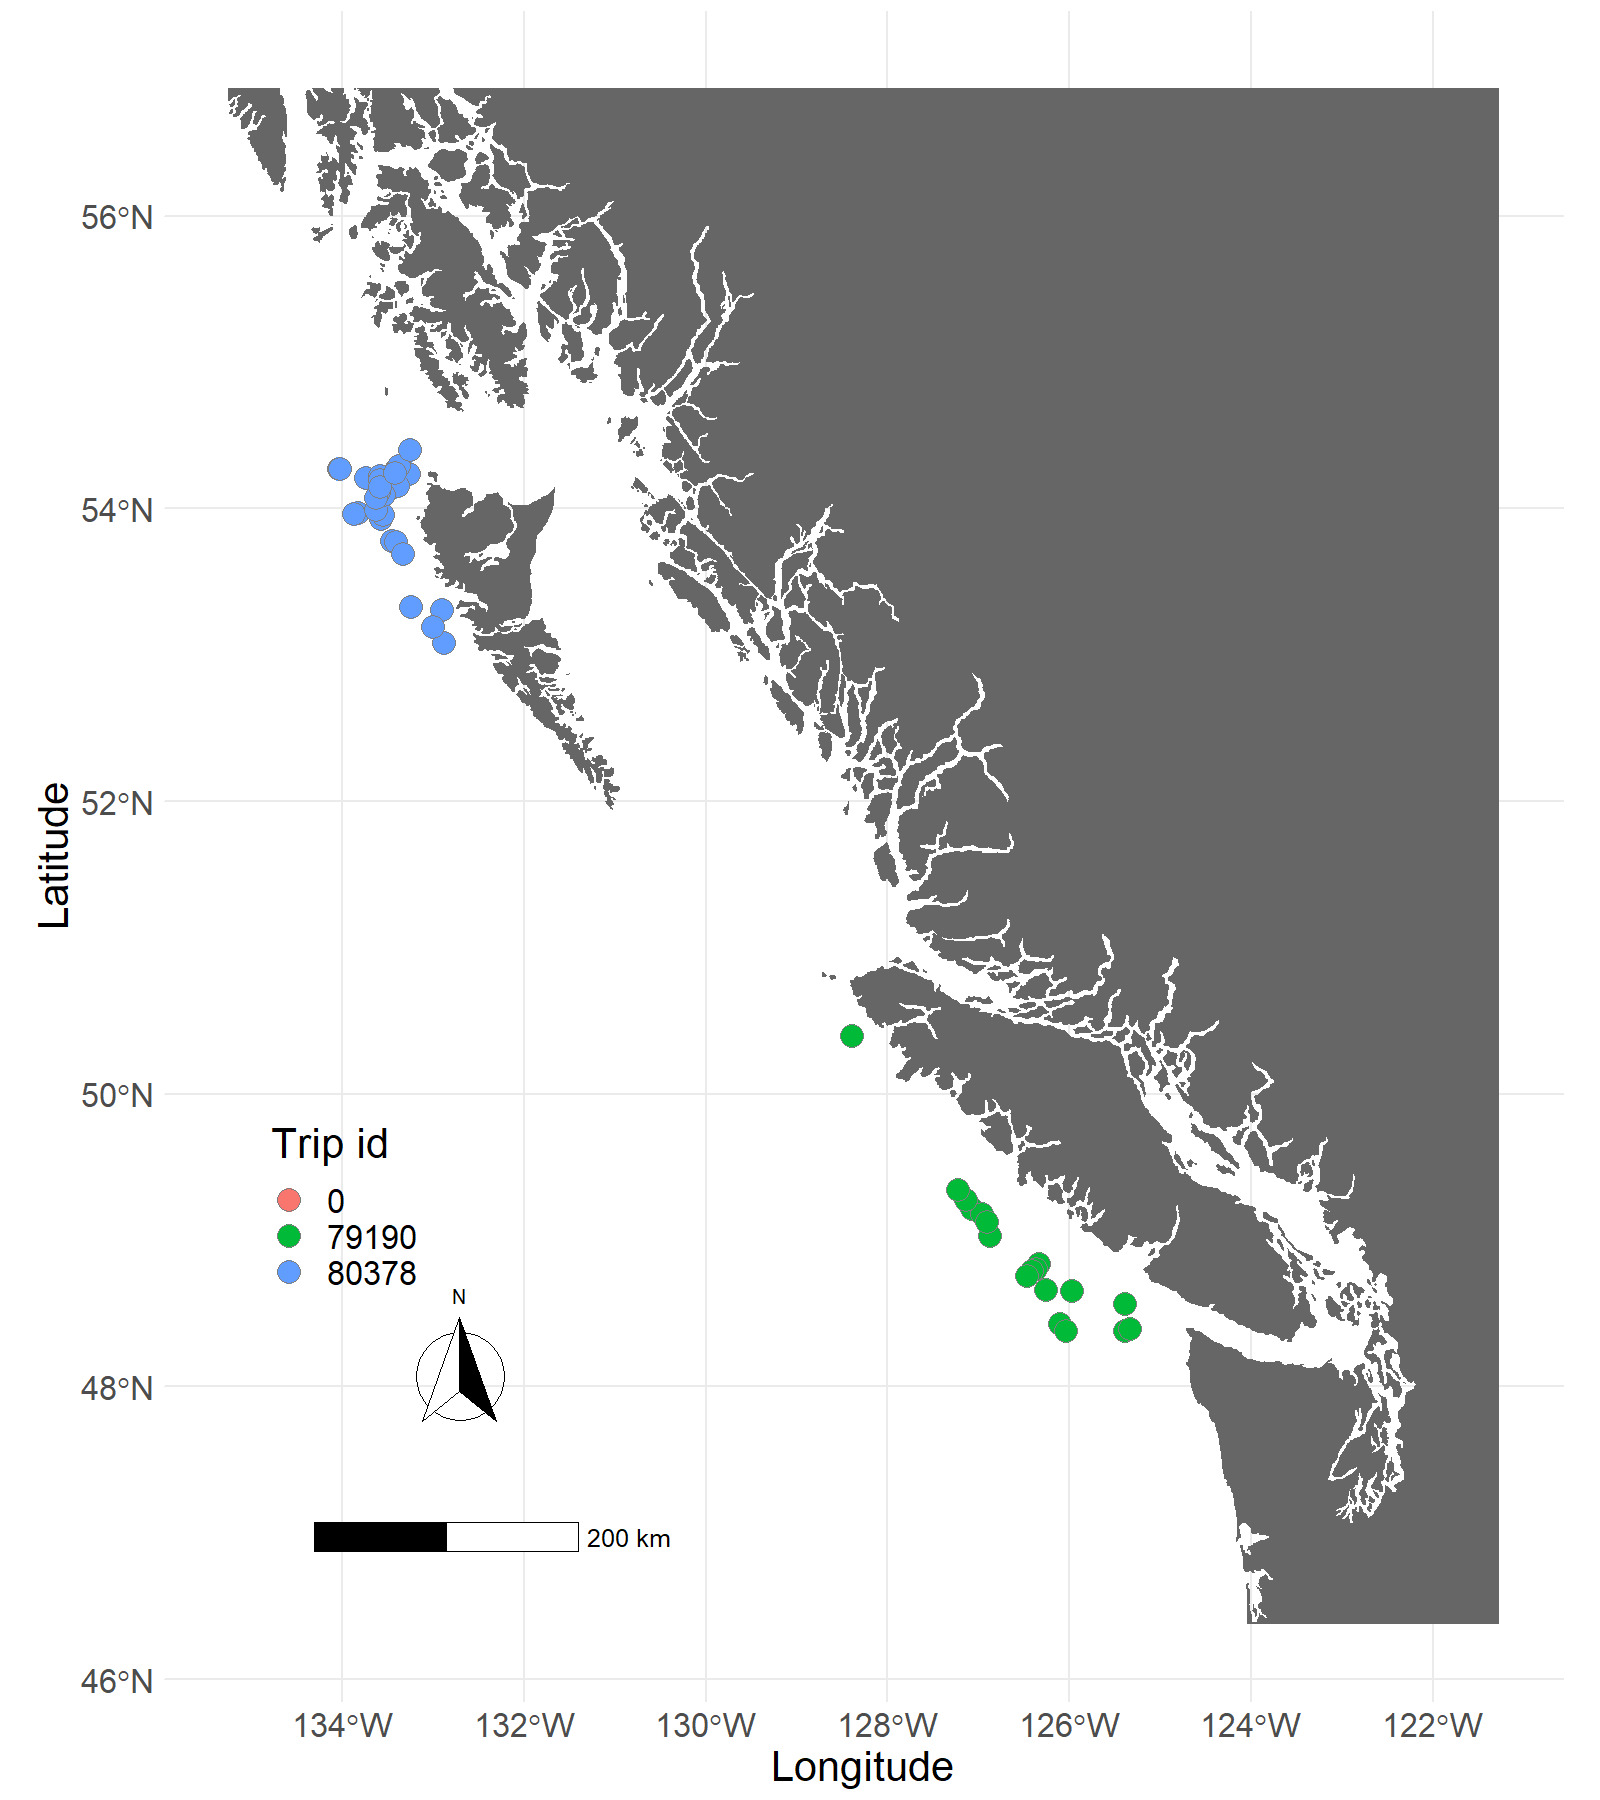
\includegraphics[width=6in]{C:/github/sablehead/figures/Figure1}}{Figure \ref{fig:figure1}} 

}

\caption{Sample locations.}\label{fig:figure1}
\end{figure}

\begin{figure}[htb]

{\centering \pdftooltip{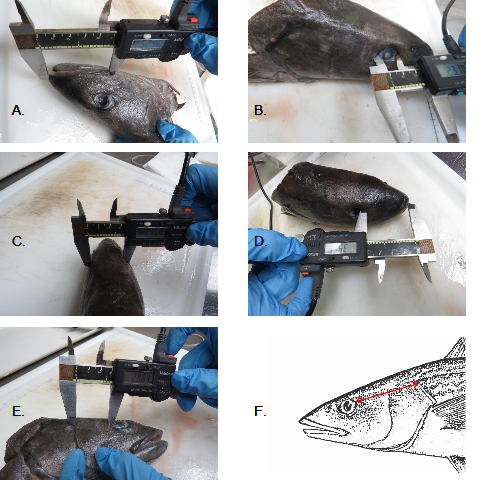
\includegraphics[width=6in]{C:/github/sablehead/figures/Figure2}}{Figure \ref{fig:figure2}} 

}

\caption{A. Upper jaw measurement; B. Eye diameter measurement; C. Interorbital distance; D. Snout length; E. Post orbital to preoperculum length measurement; F. Post orbital head length.}\label{fig:figure2}
\end{figure}

\begin{figure}[htb]

{\centering \pdftooltip{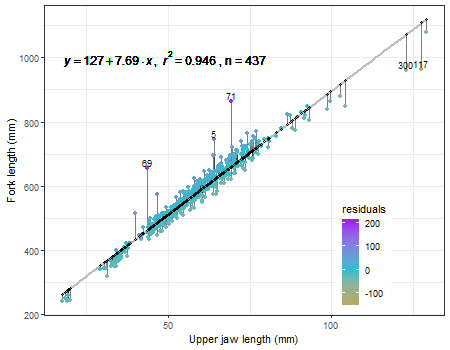
\includegraphics[width=400px,height=290px]{C:/github/sablehead/figures/Figure3}}{Figure \ref{fig:figure3}} 

}

\caption{Scatterplot upper jaw vs fork length, measurements in millimeters.}\label{fig:figure3}
\end{figure}

\begin{figure}[htb]

{\centering \pdftooltip{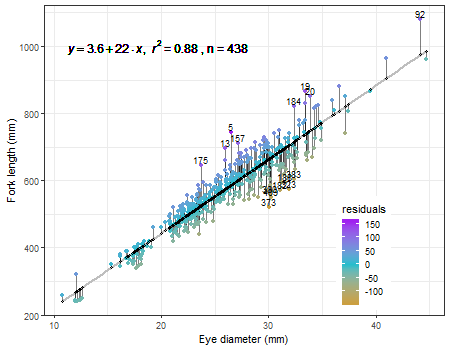
\includegraphics[width=400px,height=290px]{C:/github/sablehead/figures/Figure4}}{Figure \ref{fig:figure4}} 

}

\caption{Scatterplot eye diameter vs fork length, measurements in millimeters.}\label{fig:figure4}
\end{figure}

\begin{figure}[htb]

{\centering \pdftooltip{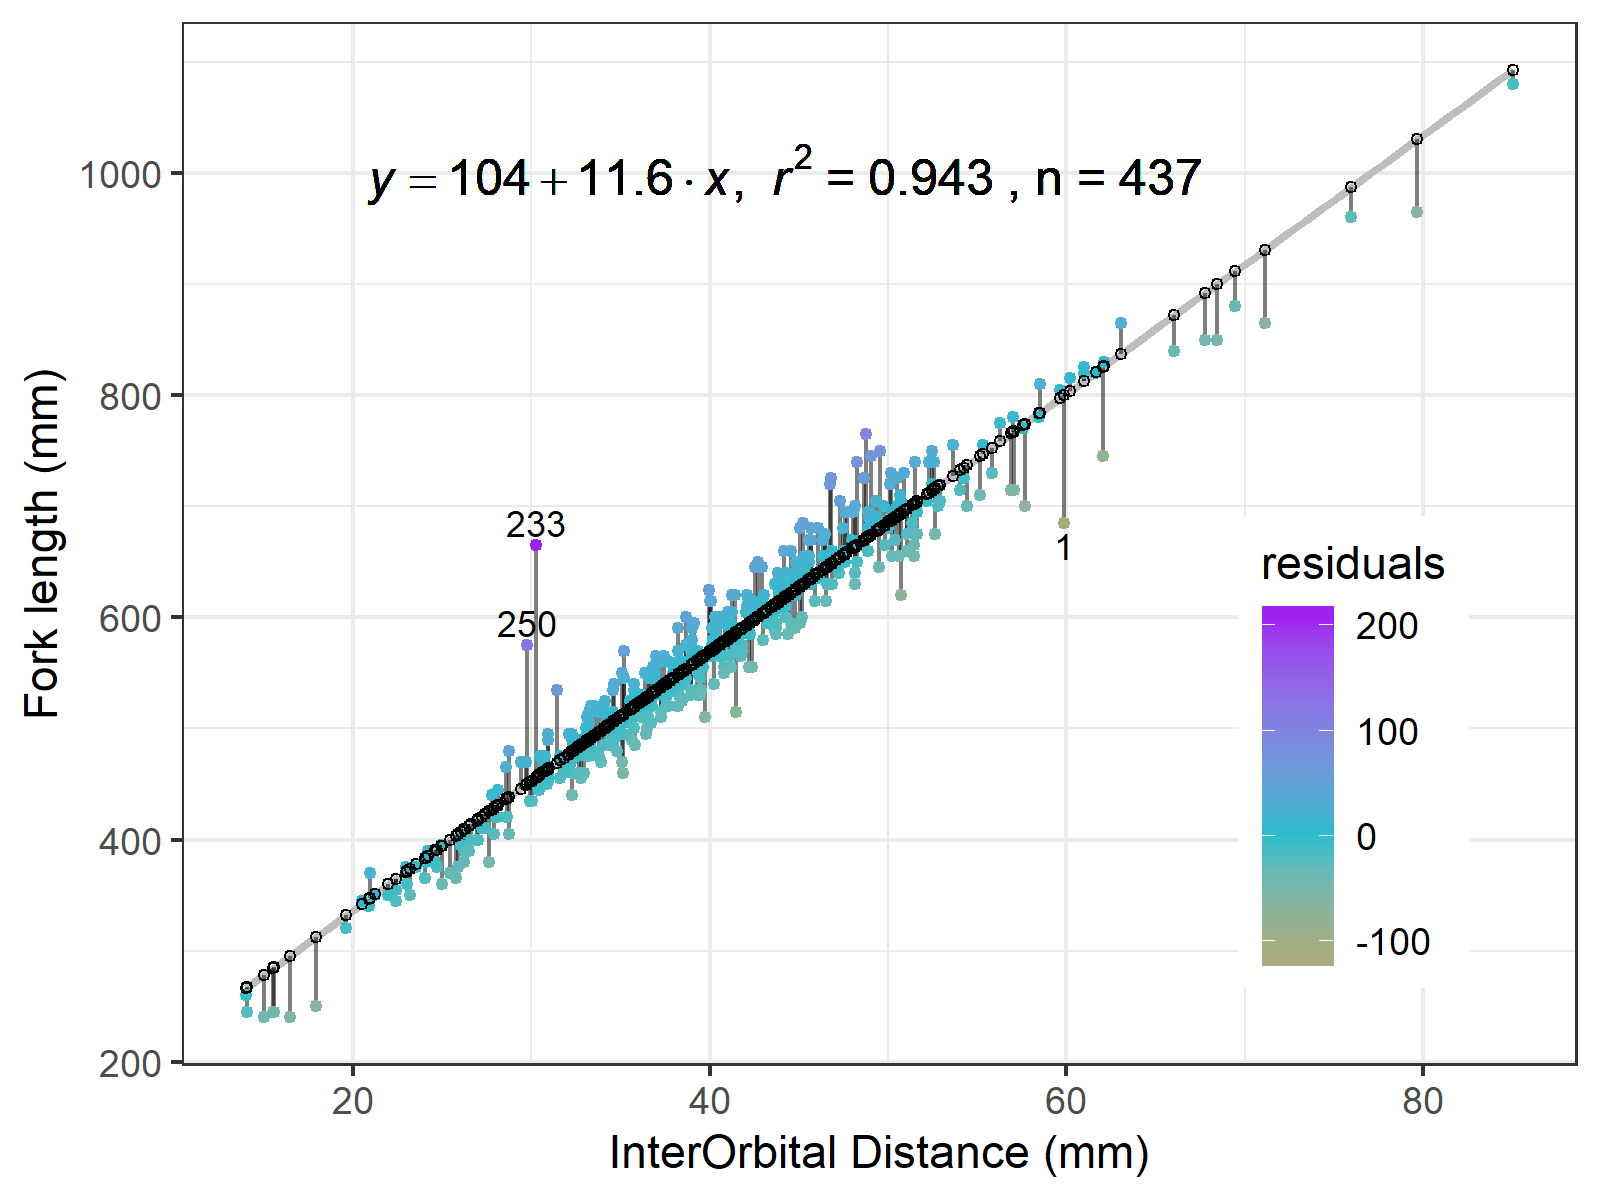
\includegraphics[width=400px,height=290px]{C:/github/sablehead/figures/Figure5}}{Figure \ref{fig:figure5}} 

}

\caption{Scatterplot interorbital vs fork length.}\label{fig:figure5}
\end{figure}

\begin{figure}[htb]

{\centering \pdftooltip{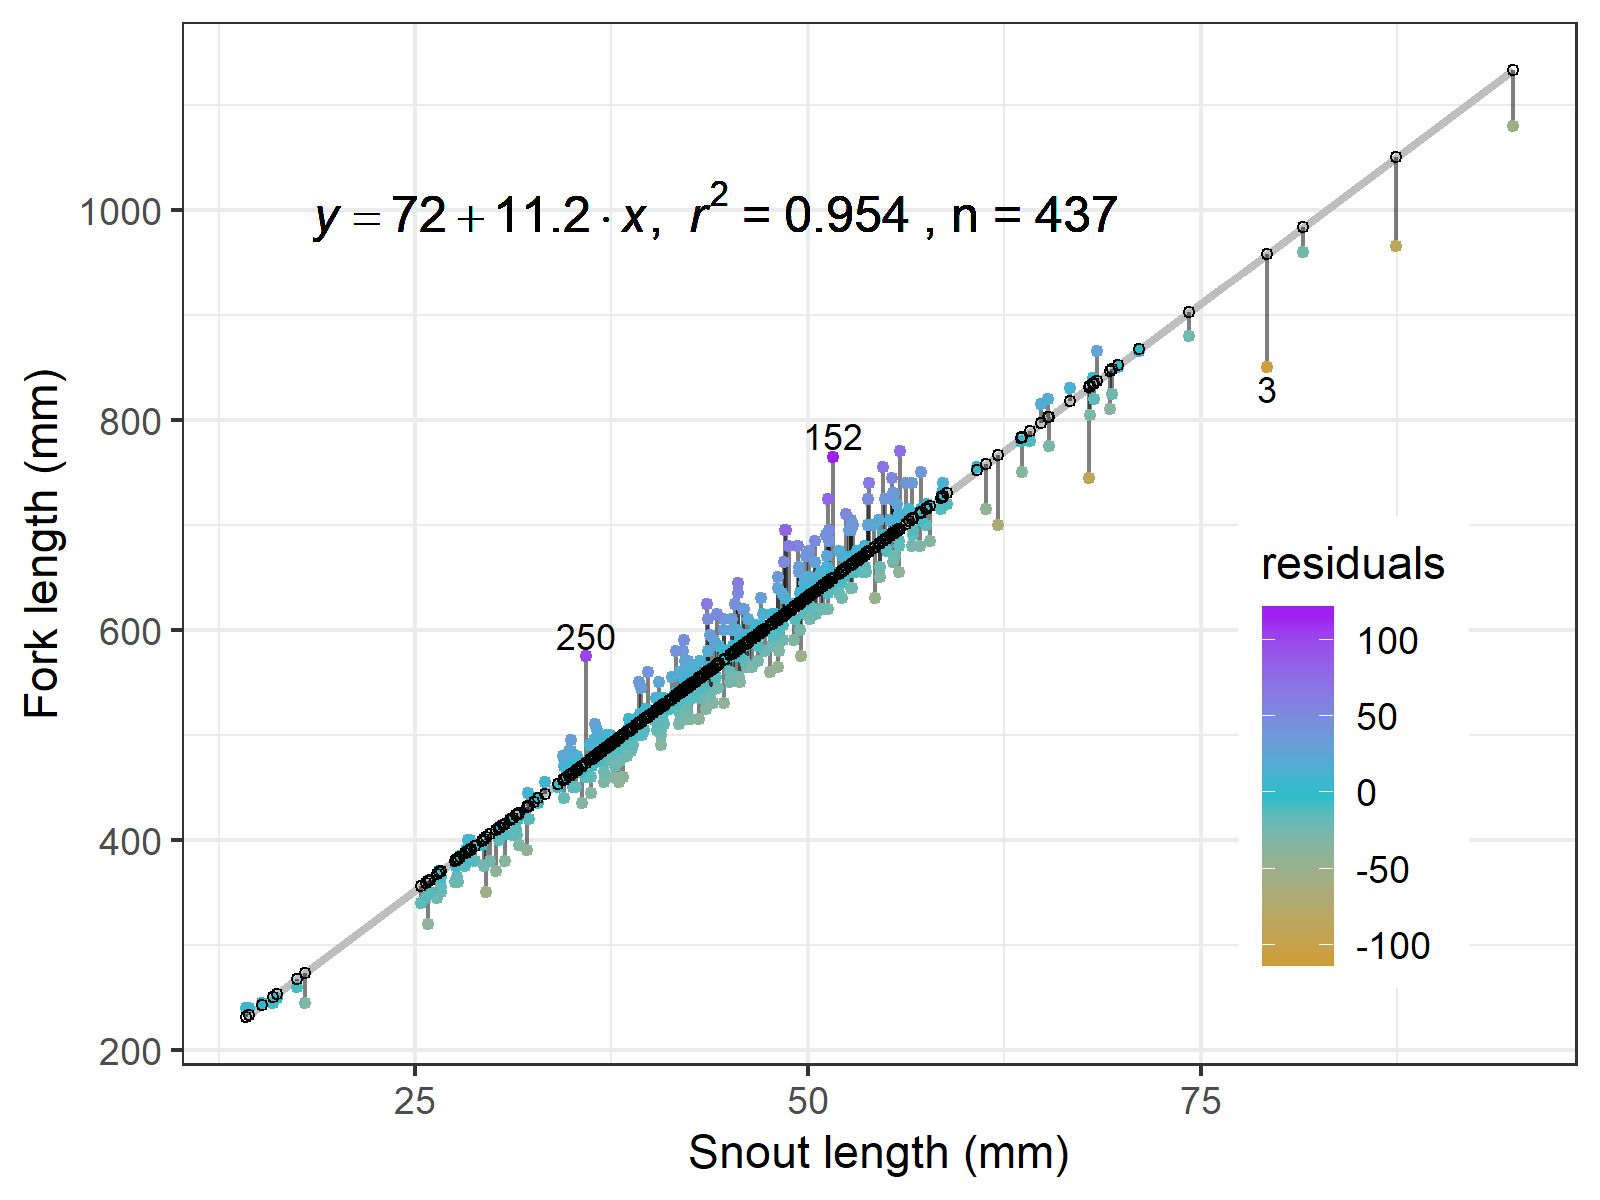
\includegraphics[width=400px,height=290px]{C:/github/sablehead/figures/Figure6}}{Figure \ref{fig:figure6}} 

}

\caption{Scatterplot snout length vs fork length.}\label{fig:figure6}
\end{figure}

\begin{figure}[htb]

{\centering \pdftooltip{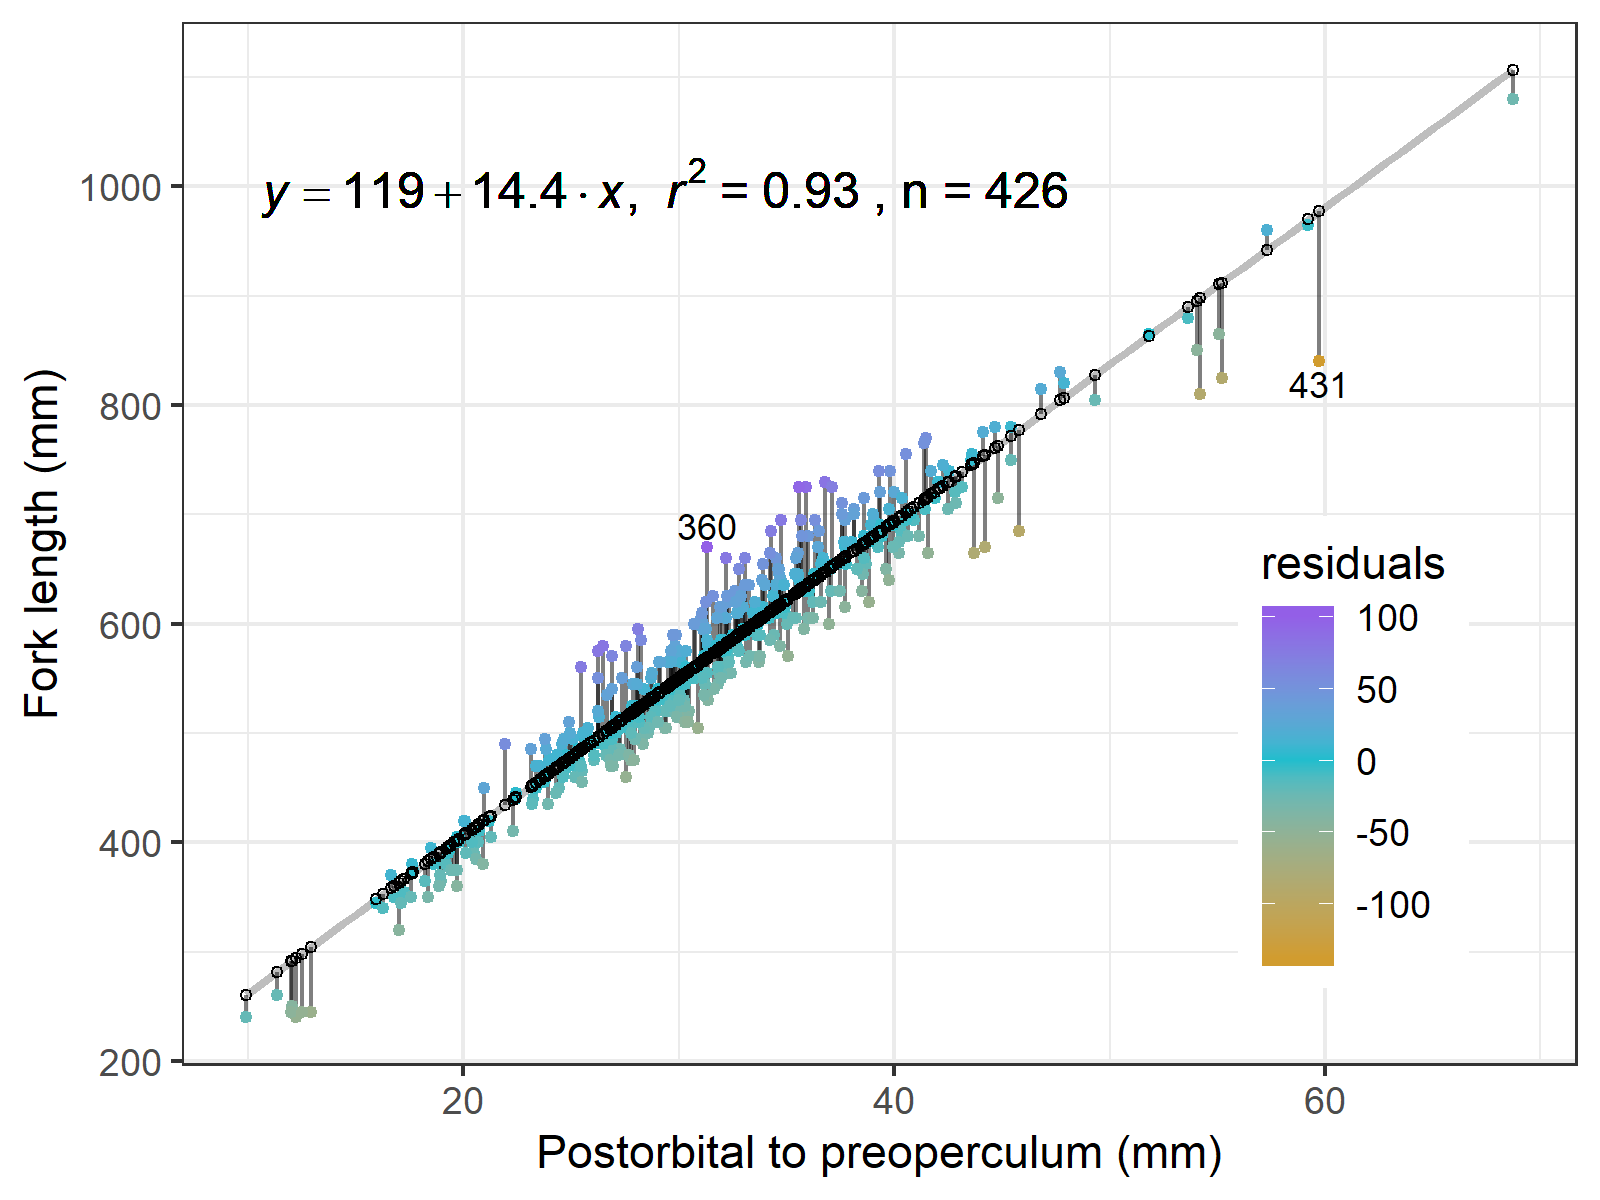
\includegraphics[width=400px,height=290px]{C:/github/sablehead/figures/Figure7}}{Figure \ref{fig:figure7}} 

}

\caption{Scatterplot post orbital to preoperculum length vs fork length.}\label{fig:figure7}
\end{figure}

\begin{figure}[htb]

{\centering \pdftooltip{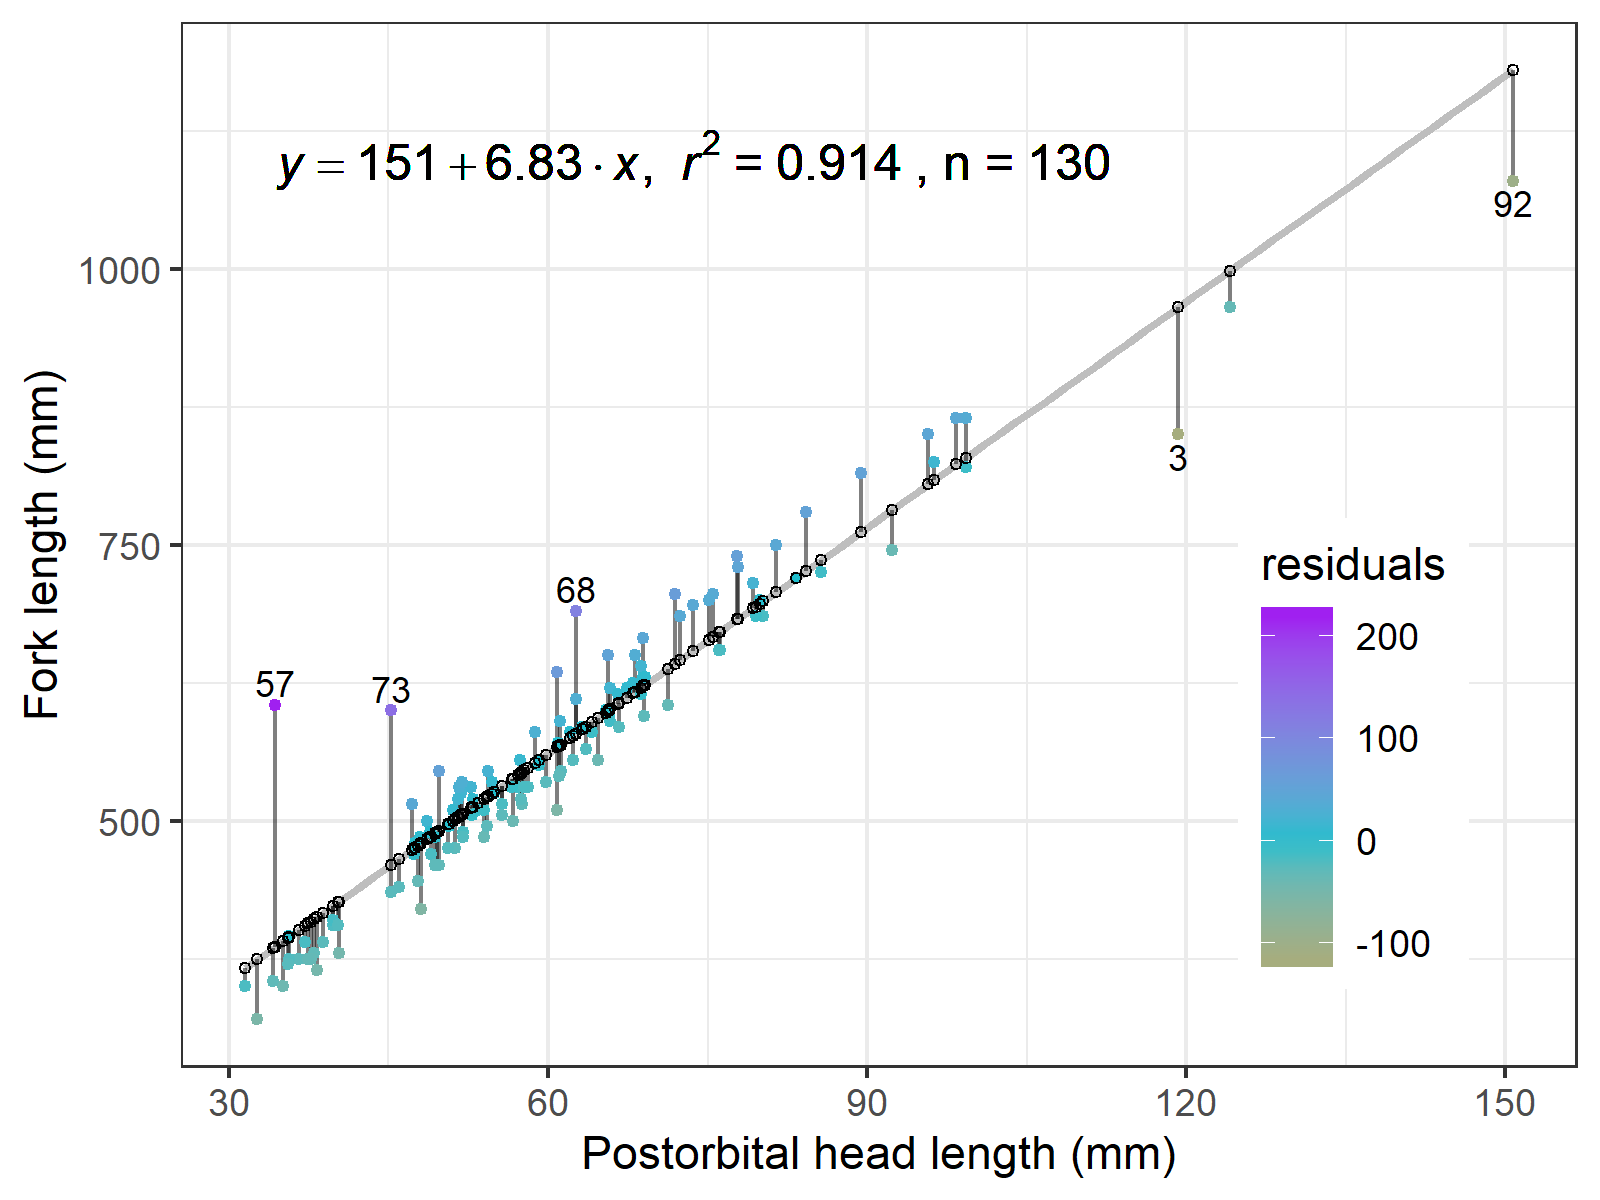
\includegraphics[width=400px,height=290px]{C:/github/sablehead/figures/Figure8}}{Figure \ref{fig:figure8}} 

}

\caption{Scatterplot of post orbital length vs fork length.}\label{fig:figure8}
\end{figure}
\clearpage
\end{document}
